\chapter{Solution of the Drift-Diffusion system}

In this chapter we introduce geometry and boundary conditions for the stationary form of system \referenzaeq{eq: full problem} and we discuss the functional iteration algorithms used to decouple the problem.

\section{Geometry and boundary conditions}

In order to close the \textit{Poisson equation} and the \textit{Drift Diffusion equation} for electrons and holes in the stationary form of problem \referenzaeq{eq: full problem}, suitable boundary conditions must be considered.

Let us consider the device domain as the union of two open disjoint subsets, $\Omega_{Si}$ (doped silicon part), and $\Omega_{ox}$ (oxide part), such that their intersection $\partial \Omega_{Si} \cap \partial \Omega_{ox} = \Gamma_{int}$ is the interface. The oxide region $\Omega_{ox}$ is assumed to be a perfect insulator so that:

\begin{equation}
\label{eq: hypotesis oxide}
\begin{array}{c}
n = p = 0 \\
\vect{J}_n = \vect{J}_p = \vect{0}.
\end{array}
\end{equation}

The device boundary $\partial \Omega$ is divided into two disjoint subsets: $\partial \Omega_{c}$ and $\partial \Omega_{a}$.
The subset $\partial \Omega_{c}$ includes the so called \textit{ohmic contacts} (with ohmic contacts we define every electrical terminal of the device on which the external input voltages are applied). Ohmic contacts are assumed to be \textit{ideal}, they are equipotential surfaces and no voltage drop occurs at the interface between the contact and the neighbouring domain. This is well represented by suitable Dirichlet boundary conditions, therefore in the following we set $\partial \Omega_{c} = \Gamma_D$ and enforce:

\begin{equation}
\label{eq: dirichlet boundary condition}
\begin{array}{cc}
\varphi = \varphi_D & \\
n = n_D & \psp{10} on \, \Gamma_D .\\
p = p_D & 
\end{array}
\end{equation}

We point that in the case of a perfect insulator domain, \referenzaeq{eq: dirichlet boundary condition} reduces to the only condition on the electrostatical potential.

\begin{figure}[!b]
\centering
\subfloat[][\label{fig: outline boundaries 1}]
{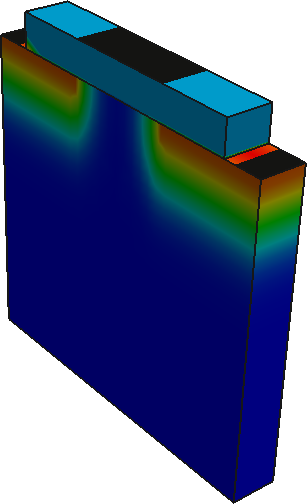
\includegraphics[scale=0.35]{Resolution/MosContacts}}
\psp{30}
\subfloat[][\label{fig: outline boundaries 2}]
{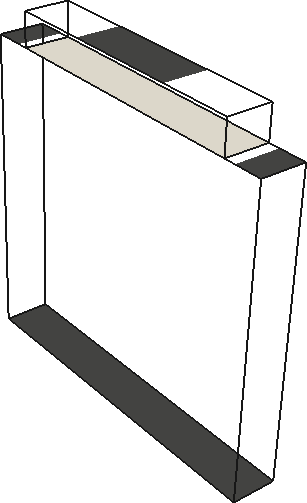
\includegraphics[scale=0.35]{Resolution/ContattiEsurface}}
\caption{(a) MOS device with net dopant concentration distributed according to a gaussian profile and $\Gamma_D$ colored in black. The oxide layer is colored in light blue. (b) Outline of the MOS device with $\Gamma_{int}$ in light gray. }
\label{fig: outline boundaries}
\end{figure}

Artificial boundaries ($\partial \Omega_a$) are needed in order to obtain a self-contained simulation domain.  On these boundaries no electric and current flux is exchanged with the surrounding environment, this fact being well represented by homogeneous Neumann boundary conditions ($\partial \Omega_a = \Gamma_N$):

\begin{equation}
\label{eq: neumann boundar condition}
\begin{array}{cc}
\vect{D}\cdot \vect{n} = 0 & \\
\vect{J}_n \cdot \vect{n} = 0 & \psp{10} on \, \Gamma_N \\
\vect{J}_p \cdot \vect{n} = 0 & 
\end{array}
\end{equation}
where $\vect{n}$ is the outward unit normal vector defined over $\partial \Omega$. 
As we noted before on $\partial \Omega_{ox} \cap \Gamma_N$ condition \referenzaeq{eq: neumann boundar condition} is reduced to the first equation.

When oxide is present the silicon boundaries for continuity equations become

\begin{equation}
\begin{array}{c}
\Gamma_{D,Si} = \Gamma_D \cap \partial \Omega_{Si} \\
\Gamma_{N,Si} = \Gamma_N \cap \partial \Omega_{Si} \cup \Gamma_{int}.
\end{array}
\end{equation}

\figref{fig: outline boundaries} shows an example of boundary setting for a MOS device: in \figref{fig: outline boundaries 1} contacts are colored in black and in \figref{fig: outline boundaries 2} with light gray we indicate the interface between oxide and silicon.

Thermodynamical equilibrium and charge neutrality are the physical characteristic of an ideal contact. These conditions correspond to the following algebraic system for $n_D$ and $p_D$:

\begin{equation}
\label{eq: systemo for dirichlet condition}
\left\{
\begin{array}{lcl}
p_Dn_D & = &n_i^2 \\
p_D -n_D +N_D^+-N_A^- & = & 0 
\end{array}
\right. .
\end{equation}

Solving \referenzaeq{eq: systemo for dirichlet condition} on $\Gamma_{D,Si}$ we have:

\begin{equation}
n_D = \dfrac{D + \sqrt{D^2+4n_i^2}}{2}
\end{equation}
\begin{equation}
p_D = \dfrac{-D + \sqrt{D^2+4n_i^2}}{2}
\end{equation}
where $D := N_D^+ -N_A^-$ is the net doping concentration. Furthermore  at each contact, the quasi Fermi potential levels of silicon are aligned with the external applyed voltage $V_{ext}$

\begin{equation}
\varphi_n=\varphi_p=\varphi_f=V_{ext}.
\end{equation}
where $\varphi_f = - E_f / q$ is the unique quasi Fermi potential level defined at the contacts.
As a consequence, we can easily determine potential condition on $\Gamma_{D,Si}$ using \referenzaeq{eq: n density mb} and \referenzaeq{eq: p density mb}

\begin{equation}
\varphi_D = \varphi_f + V_{th}\ln\left( \dfrac{n_D}{n_i} \right) = \varphi_f - V_{th}\ln\left( \dfrac{p_D}{n_i} \right)
\end{equation}

 When $\Omega_{ox} \neq \varnothing$ we set $\varphi_D$ equal to the external applyed voltage on $\Gamma_D / \Gamma_{D,Si}$.


The stationary form of \referenzaeq{eq: full problem} can be now written in closed form as:
 

\begin{equation}
\label{eq: system closed}
\begin{array}{rcll}
- \Delta \epsilon \varphi - q(p-n) & =  & qD & in \, \Omega = \Omega_{ox} \cup \Omega_{Si}\\
\varphi & = & \varphi_D & on \, \Gamma_D \\
\nabla \varphi \cdot \vect{n} & = & 0 & on \, \Gamma_N 
\\
\\
\nabla \cdot ( q\mu_n n \nabla \varphi - qD_n \nabla n ) & = & - qR & in \, \Omega_{Si}\\
n & = & n_D & on \, \Gamma_{D,Si} \\
\nabla n \cdot \vect{n} & = & 0 & on \, \Gamma_{N,Si}
\\
\\
\nabla \cdot (- q\mu_p p \nabla \varphi - qD_p \nabla p )& = & -qR& in \, \Omega_{Si}\\
p & = & p_D & on \, \Gamma_{D,Si} \\
\nabla p \cdot \vect{n} & = & 0 & on \, \Gamma_{N,Si}.
\end{array}
\end{equation}

The highly nonlinear coupled nature of system	\referenzaeq{eq: system closed} makes an analytical treatment very difficult, if not even impossible. For this reason, numerical schemes must be used to  compute an approximate solution. 


\section{Iteration algorithms}

 The most used algorithms for the iterative treatment of \referenzaeq{eq: system closed} are \textit{the fully coupled Newton's method} and \textit{the decoupled Gummel map}. System \referenzaeq{eq: system closed} can be written in compact form as

\begin{equation}
\label{eq: abstract problem fully}
\vect{F(U)}=\vect{0}
\end{equation}

where

\begin{equation}
\label{eq: functional operator}
\vect{U}:=[\varphi,n,p]^T, \psp{30} \vect{F(U)}:=\left[ \begin{array}{c}
F_1(\vect{U}) \\
F_2(\vect{U}) \\
F_3(\vect{U})
\end{array}
\right]
\end{equation}

having set:

\begin{align*}
F_1(\vect{U}) & = \nabla \cdot (-\epsilon \nabla \varphi) - q(p-n+D) \\
F_2(\vect{U}) & = \nabla \cdot ( q\mu_n n \nabla \varphi - qD_n \nabla n )+qR \\
F_3(\vect{U}) & = \nabla \cdot (- q\mu_p p \nabla \varphi - qD_p \nabla p )+qR.
\end{align*}

Problem \referenzaeq{eq: abstract problem fully} is the generalization of the search of a zero for a real function $f:\mathbb{R}\rightarrow\mathbb{R}$. Because the vector function $\vect{F}$ is a nonlinear differential operator, the associated problem which we intend to solve is: given a functional space $V$ and the operator $\vect{F}:V\rightarrow V$, find $\vect{U}\in V$ such that \referenzaeq{eq: abstract problem fully} is satisfied.

In our application, the function space $V$ is typically a subset of the Sobolev space  $[H^1(\Omega)]^d$ (where $d$ is the number of component of $\vect{F}$). 
The general form of a Sobolev space for an integer $m\geq 0$ is

\begin{equation}
\label{space: Hm}
H^m(\Omega) := \left\{ v : D^{\alpha}v\in L^2(\Omega),\forall |\alpha|\leq m \right\}.
\end{equation}

where $L^2(\Omega)$ is the space of square integrable functions on $\Omega$ defined as

\begin{equation}
\label{space: L2}
L^2(\Omega) := \left\{ v : \int_{\Omega} |v|^2 d\,\Omega =||v||^2_{L^2(\Omega)}<+\infty \right\}.
\end{equation}

On these space, we shall use the semi-norm

\begin{equation}
\label{eq: semiorm sobolev}
|v|_{m,\Omega}^2 = \sum_{|\alpha|=m} ||D^{\alpha}v||^2_{L^2(\Omega)}
\end{equation}

and the norm

\begin{equation}
\label{eq: norm sobolev}
||v||_{m,\Omega}^2 = \sum_{k\leq m} |D^{\alpha}v|^2_{k,\Omega}.
\end{equation}

We shall also need to consider functions that vanish on either the entire or a part of the boundary:

\begin{align}
& H^1_0 :=  \left\{   v : v \in H^1(\Omega), v|_{\partial \Omega} = 0\right\} \label{space: h1 zero} \\
& H^1_{0,\Gamma_D} :=  \left\{   v : v \in H^1(\Omega), v|_{\Gamma_D} = 0\right\} \label{space: h1 zero gamma}
\end{align} 

For $v \in H^1_0(\Omega),H^1_{0,\Gamma_D}(\Omega)$ we have the \textit{Poincar\'e - Friedrich's inequality} \cite{salsa:EDP}

\begin{equation}
\label{eq: poincarre inequality}
|v|_{0,\Omega} \leq C(\Omega) |v|_{1,\Omega}
\end{equation}

from which it follows that the seminorm $|\cdot |_{\,\Omega}$ is actually a norm in $H^1(\Omega)$, equivalent to $||\cdot ||_{1,\Omega}$.

The above function spaces (for a more detailed description see \cite{Adams:SobolevSpaces}) are used widely in the remainder of this work, especially during the well-posedness analysis as reported in Chapter \ref{chap: finite element}.


\subsection{Newton's method}

\begin{Definizione}[Frech\`et differentiability]
Let be $X$ and $Y$ two vector spaces. Given $f,g \in X$ and a functional $F:X\rightarrow Y$, the functional $F$ is Frech\'et differentiable if there exists a linear bounded operator $A_f:X\rightarrow Y$ such that

\begin{equation}
\lim_{||g||\to 0}\dfrac{||F(f+g)-F(f)-A_f(g)||_Y}{||g||_X} = 0 ,
\end{equation}
where $||\cdot ||_X$ and $||\cdot ||_Y$ are the norms on $X$ and $Y$ respectively.
If the above limit exists, we write $DF(f)=A_f$ and call it the Frech\'et derivative of $F$ at $f$.
\end{Definizione}


Considering the functional operator \referenzaeq{eq: functional operator} we can easily compute the associated \textit{Jacobian matrix} $\vect{F}'$, whose $(i,j)-th$ entry represents the Frech\'et derivative of the $i-th$ row of the non linear operator with respect to the $j-th$ variable, defined as

\begin{equation}
\vect{F}'_{ij}(\vect{U})[\vect{V}]_j := \lim_{\eta \to 0}\dfrac{F_i(\vect{U}+\eta [\vect{V}]_j)-F_i(\vect{U})}{\eta}  \psp{10} \vect{V} \in V
\end{equation}

where $[\vect{V}]_j \in V$ is the projection  of  $\vect{V}$ in the $j-th$ direction. 

$\vect{F}'_{ij}(\cdot)$ is a linear operator from $V$ into the space $L(V,V)$ of linear continuos functionals from $V$ into $V$, while $\vect{F}'_{ij}(\vect{U})$ is the Frech\'et derivative of the functional $F_i$ with respect the variable $[\vect{U}]_j$.

According to the above definitions the Newton method reads as follows:


\mybox{
Let $X, Y$ be two vector spaces and $\vect{F}:X\rightarrow Y$ a function operator Frech\`et differentiable, given an initial datum $\vect{U}^0\in X$ and $toll>0$, for all $k\geq 0$ solve the following linear problem:

\begin{equation}
\label{eq: abstract newton's method}
\begin{array}{c}
\vect{F'}(\vect{U}^k)\delta\vect{U}^k=-\vect{F}(\vect{U}^k) \\
\vect{U}^{k+1} = \vect{U}^k + \delta \vect{U}^k
\end{array}
\end{equation}

 until $||\vect{F}(\vect{U}^{k+1})||_Y<toll$. 
}{\textbf{Newton's method}}
\vspace{0.3cm}
The application of Newton's method has transformed the original problem \referenzaeq{eq: abstract problem fully} into the \textit{fixed-point problem} of finding $\vect{U} \in V$ such that

\begin{equation}
\label{eq: fixed point U}
\vect{U} = T_{\vect{F}}(\vect{U})
\end{equation}

where 

\begin{equation}
\label{eq: iteration function}
T_{\vect{F}}(\vect{U}) = \vect{F}'(\vect{U})^{-1}(\vect{F}'(\vect{U})\vect{U}-F(\vect{U}))
\end{equation}

is the \textit{iteration function} associated with the Newton method.
The main result about the convergence of this method is the follow \cite{Ortega:IterNonlinearEq}

\begin{Teorema}
\label{theorem: newton convergence}
Let  $\vect{U}\in V$ be a solution of problem \referenzaeq{eq: abstract problem fully}. Assume that $\vect{F'}$ is Lipschitz continuos in the ball $\mathcal{B}(\vect{U},\delta)$, i.e., that there exists  $K>0$ such that:
\begin{equation}
||\vect{F'}(\vect{v})-\vect{F'}(\vect{z})||_{L(V,V)} \leq K ||\vect{v}-\vect{z}||_V \psp{10} \forall \vect{v},\vect{z} \in \mathcal{B}(\vect{U},\delta), \, \vect{v}\neq \vect{z}
\end{equation}
Then there exists in correspondence $\delta '>0$, with $\delta '\leq\delta$, such that for all $\vect{U}^0 \in \mathcal{B}(\vect{U},\delta ')$ the sequence $\left\{ \vect{U}^k \right\}$ generated by \referenzaeq{eq: abstract newton's method} converges quadratically to $\vect{U}$, i.e., there exists $C>0$ such that, for a suitable $k_0\geq 0$ we have:
\begin{equation}
\label{eq: convergece newton}
||\vect{U}-\vect{U}^{k+1}||_V\leq C||\vect{U}-\vect{U}^k||_V^2 \psp{15} \forall k\geq k_0
\end{equation}
\end{Teorema}


\subsection{Fully coupled Newthon's method}


If we consider the linearization of system \referenzaeq{eq: system closed} the Jacobian matrix of the Newton method is a 3x3 matrix and the associated problem is

\begin{equation}
\label{eq: NLP algorithm matrix}
\left[
\begin{array}{ccc}
F_{1,\varphi} & F_{1,n} & F_{1,p} \\
F_{2,\varphi} & F_{2,n} & F_{2,p} \\
F_{3,\varphi} & F_{3,n} & F_{3,p} \\
\end{array}
\right]
\left[
\begin{array}{c}
\delta \varphi  \\
\delta n  \\
\delta p 
\end{array}
\right]
=
\left[
\begin{array}{c}
-F_1(\varphi,n,p) \\
-F_2(\varphi,n,p)\\
-F_3(\varphi,n,p)
\end{array}
\right] .
\end{equation}


 Each row of the above matrix is a PDE that can be discretized using the FEM. Denoting by $N_{dof}$ the number of degrees of freedom (dofs) to represent $\delta \varphi$, $\delta n$ and $\delta p$ we see that the structure of the discrete problem associated with \referenzaeq{eq: NLP algorithm matrix} is the following linear algebraic system

\begin{equation}
\left[
\begin{array}{ccc}
\vect{K}_{1,\varphi} & \vect{K}_{1,n} & \vect{K}_{1,p} \\
\vect{K}_{2,\varphi} & \vect{K}_{2,n} & \vect{K}_{2,p} \\
\vect{K}_{3,\varphi} & \vect{K}_{3,n} & \vect{K}_{3,p} \\
\end{array}
\right]
\left[
\begin{array}{c}
\delta \varphi  \\
\delta n  \\
\delta p 
\end{array}
\right]
=
\left[
\begin{array}{c}
-\vect{F}_1(\varphi,n,p) \\
-\vect{F}_2(\varphi,n,p)\\
-\vect{F}_3(\varphi,n,p)
\end{array}
\right]
\end{equation}
where each matrix $\mathbf{K}$ is a block of size $N_{dof} \times N_{dof}$. 
This implies that at every iteration step we have to solve a linear problem of $3 \times N_{dof}$ variables.
Moreover, to ensure convergence of the Newton iterative process, it is important to provide a very good initial guess vector $[\varphi^0,n^0,p^0]$. Because the problem variables have different orders of magnitude and the Jacobian matrix is often quite ill-conditioned, appropriate scaling and balancing techniques are needed in order to avoid problems associated with round-off error. 


\subsection{Gummel map algorithm}

In 1964 H. K. Gummel proposed an original and alternative to  \referenzaeq{eq: NLP algorithm matrix} approach in order to solve system \referenzaeq{eq: system closed} in a semiconductor device in one spatial dimension \cite{GummelMap}.
The main idea of the algorithm is to move the nonlinearity to the Poisson equation only, and once obtained the electric potential profile, both continuity equations are solved in linear form. This is possible if we consider the Maxwell-Boltzmann approximation for electrons \referenzaeq{eq: n density mb} and holes \referenzaeq{eq: p density mb} obtaining

\begin{equation}
F_1(\varphi)  =  \nabla \cdot (-\epsilon \nabla \varphi) - q(n_i(e^{(\varphi_p-\varphi)/V_{th}}-e^{(\varphi-\varphi_n)/V_{th}})+D) .
\end{equation}

\begin{figure}[!h]
\begin{center}
\begin{tikzpicture}
[scale=1.2]

\tikzstyle{NLP}=[rectangle,text width=3cm, align=center,draw, fill=gray!40];
\tikzstyle{DD}=[rectangle,text width=3cm,align=center,draw,fill=gray!10];
\tikzstyle{Normal}=[rectangle,fill=white];
\tikzstyle{CYC}=[diamond,draw];
\useasboundingbox (0,1) rectangle (8,9.5);
\draw [thick] (-0.5,1.0) rectangle (8.5,9.5);
%main boxes
\node [Normal] (v0) at (1,8) {$[\varphi,n,p]_{start}$};
\node [NLP] (v1) at (4,8) {\large NLP};
\node [CYC] (v2) at (4,7) {\small k};
\node [DD] (v3) at (4,5.5) {\large DD electrons};
\node [DD] (v4) at (4,4.0) {\large DD holes};
\node [CYC] (v5) at (4,2.5) {\small i};

%collegamenti
\draw [thick,->] (v0) -- (v1);
\draw [thick,->] (v1) -- (v2);
\draw [thick,->] (v2) -- (v3);
\draw [thick,->] (v3) -- (v4);
\draw [thick,->] (v4) -- (v5);
\draw [thick,->] (v5)--(7,2.5)--(7,9)--(4,9)--(v1);
\draw [thick,->] (v2)--(6,7)--(6,8)--(v1);
\draw [thick,->] (v5)--(4,1.5);

%note
\node [Normal] (v6) at (5.5,7.3) {$\varphi^{k+1}$};
\node [Normal] (v6) at (4.5,6.2) {$\varphi_{i+1}$};
\node [Normal] (v6) at (4.5,4.7) {$n_{i+1}$};
\node [Normal] (v6) at (4.5,3.2) {$p_{i+1}$};
\node [Normal] (v0) at (5.0,1.8) {$[\varphi,n,p]_{end}$};
\end{tikzpicture}
\caption{Flow chart of Gummel algorithm.}
\label{fig: gummel map}
\end{center}
\end{figure}


The Gummel algorithm is represented by the following iteration.

\mybox{

\begin{itemize}
\setlength{\itemsep}{15pt}

\item[\bf 0.] Give a suitable initial condition for $\varphi^0$ and set a positive parameter $toll_{GM}>0$ (Gummel Map tollerance)

\item[\bf 1.] Fix a positive parameter $toll_{NLP}>0$ (Non Linear Poisson tolerance), solve the linearized Non Linear Poisson equation (NLP) in $\Omega$ using the Newton method until $||F_1(\varphi^{k+1})||>toll_{NLP}$:



\begin{equation}
\label{eq: newton step NLP linear}
\begin{cases}

\nabla \cdot (-\epsilon_{Si} \nabla \delta\varphi^k) 
+   \dfrac{1}{V_{th}} \sigma_{Si}^k\delta\varphi^k 
 =  f_{Si}^k & in \psp{3} \Omega_{Si}
  \\
\nabla \cdot (-\epsilon_{ox} \nabla \delta\varphi^k) =  f_{ox}^k & in \psp{3} \Omega_{ox} 
\\
\delta \varphi^k = 0 & on \psp{3} \Gamma_D 
\\
\nabla \delta \varphi^k \cdot \vect{n} = 0 & on \psp{3} \Gamma_N
\\
\varphi^{k+1}=\varphi^k+\delta \varphi^k
\end{cases} 
\end{equation}

having set:

\vspace{-0.6cm}

\begin{align*}
\sigma_{Si}^k(\varphi^{k}) & = qn_i \left[ e^{(\varphi_p-\varphi^k)/V_{th}}-e^{(\varphi^k-\varphi_n)/V_{th}} \right]
\\
f_{Si}^k(\varphi^k) & = \nabla \cdot (-\epsilon \nabla \varphi^k) + qn_i \left[ e^{(\varphi_p-\varphi^k)/V_{th}}-e^{(\varphi^k-\varphi_n)/V_{th}}  + D \right]
\\
f_{ox}^k(\varphi^k) & = \nabla \cdot (-\epsilon \nabla \varphi^k) . 
\end{align*}

\item[\bf 2.] Solve the Linear Electron Continuity Equation (LEC):

\vspace{-0.5cm}

\begin{equation}
\label{eq: LEC system}
\begin{cases}
 \nabla \cdot ( q\mu_n n \nabla \varphi^i - qD_n \nabla n ) = -qR(n^{i-1},p^{i-1}) & in \psp{3} \Omega_{Si}
 \\
 n = n_D & on \psp{3} \Gamma_{D,Si}
 \\
 \nabla n \cdot \vect{n} = 0 & on \psp{3} \Gamma_{N,Si}
\end{cases}
\end{equation}

\item[\bf 3.] Solve the Linear Hole Continuity Equation (LHC):

\vspace{-0.5cm}

\begin{equation}
\label{eq: LHC system}
\begin{cases}
\nabla \cdot (- q\mu_p p \nabla \varphi^i - qD_p \nabla p ) =  -qR(n^{i-1},p^{i-1}) & in \psp{3} \Omega_{Si}
\\
 p = p_D & on \psp{3} \Gamma_{D,Si}
 \\
 \nabla p \cdot \vect{n} = 0 & on \psp{3} \Gamma_{N,Si}
\end{cases}
\end{equation}

\item[\bf 4.] If $\max\{||\varphi^i-\varphi^{i-1}||_{L^{\infty}},||p^i-p^{i-1}||_{L^{\infty}},||n^i-n^{i-1}||_{L^{\infty}}\}>toll_{GM}$ restart from step (1).


\end{itemize}

}{\textbf{Decoupled Gummel map.}}

 \figref{fig: gummel map} shows a flow chart of the Gummel algorithm where $k$ is the iteration step of the inner loop, while $i$ is the iteration step of the Gummel Map.
 
For the Gummel map, similar result as \teoref{theorem: newton convergence}  can be found in \cite{Jerome:AnalyCharTran}, but the convergence rate is linear. However heuristic experience often shows superlinear convergence behaviour.

There are several advantages which make Gummel map algorithm better than the Fully Coupled Newton's Method, indeed simulations experience shows that the Gummel process is much more insensitive to the choice of the initial guess than Newton's method. This is particularly important in multidimensional problems where it is far from trivial to design a good starting point for initializing the iterative procedure. Another attractive feature is the reduced computational effort and memory cost: at each iteration step the Gummel algorithm requires the successive solution of three problems, each one of size equal to $N_{dof}\times N_{dof}$.


Let us discuss again steps 2-3 of \textit{Decoupled Gummel map}. According with \referenzaeq{eq: generic RG} the general R/G phenomenon can be separated in a reaction term and a force term (except for the II which is only a force term contribution). 
Considering

\begin{equation}
\label{eq: real Rn and Rp}
\begin{array}{rcl}
R_n^{i-1}(n) & = \sigma_n^{i-1} n - f^{i-1} \\
R_p^{i-1}(p) & = \sigma_p^{i-1} p - f^{i-1} \\
\end{array}
\end{equation}

where


\begin{equation}
\begin{array}{c}
\sigma_n  = \dfrac{p^{i-1}}{F(p^{i-1},n^{i-1})} \psp{15} \sigma_p   = \dfrac{n^{i-1}}{F(p^{i-1},n^{i-1})} \\
f  = \dfrac{n_i^2}{F(p^{i-1},n^{i-1})}
\end{array}
\end{equation}

we can rewrite systems \referenzaeq{eq: LEC system} and \referenzaeq{eq: LHC system} as:

\begin{equation}
\label{eq: LEC system new}
\begin{cases}
 \nabla \cdot ( q\mu_n n \nabla \varphi^i - qD_n \nabla n ) +q\sigma_n^{i-1} n = qf^{i-1} & in \psp{3} \Omega_{Si}
 \\
 n = n_D & on \psp{3} \Gamma_{D,Si}
 \\
 \nabla n \cdot \vect{n} = 0 & on \psp{3} \Gamma_{N,Si}
\end{cases}
\end{equation}

\begin{equation}
\label{eq: LHC system new}
\begin{cases}
\nabla \cdot (- q\mu_p p \nabla \varphi^i - qD_p \nabla p ) + q\sigma_p^{i-1} p =  qf^{i-1}& in \psp{3} \Omega_{Si}
\\
 p = p_D & on \psp{3} \Gamma_{D,Si}
 \\
 \nabla p \cdot \vect{n} = 0 & on \psp{3} \Gamma_{N,Si}\, .
\end{cases}
\end{equation}


The above splitting of R/G term is called \textit{lagging approach} \cite{Jerome:AnalyCharTran} and corresponds to extend to the non-linear case the classical \textit{Jacobi} method for the iterative  solution of linear algebraic systems. Since equations are sequentially solved, it is possible take advantage of the solution at the present step. Indeed an alternative approach would be use the solution of the first solved equation to compute the R/G contribution in the second equation. In such a case, the lagging method corresponds to extend to the nonlinear case the classical \textit{Gauss-Seidel} method for the iterative solution in linear algebraic systems.


